\section{Experimental Results/Evaluation}
\label{sec:experiments}


% The Material Evolution Graph is implemented as a directed hypergraph to represent industrial transformations and material dependencies.
% \anil{structural properties: degree distribution of nodes, reachability of individual products}


\subsection{Implementation details}

Using our approach, we produced four separate \tool{}s for Germanium, Gallium, Cobalt, and Boron. For each, we started with a material or family of related materials (for example, Cobalt starts with three different related materials - see Table 1). For each, common materials were identified (within the realm of microelectronics) that require the starting material for their production. Lastly, all transformation processes necessary to produce these materials were discovered (see Table 1). Due to the time required for each iteration, the material and process identification phases for creating these four hypergraphs were limited to five iterations.

\begin{table}[h!]
\centering
{\small
\begin{tabularx}{8.5cm}{|>{\raggedright\arraybackslash}p{3.5cm}|X|X|}
\hline
\footnotesize\textbf{Starting Material(s)\newline [Node(s)] } & \footnotesize\textbf{Transformation\newline Materials\newline [Nodes]} & \footnotesize\textbf{Transformation\newline Processes\newline [Hyperedges]} \\
\hline
Germanium & 59 & 59 \\
\hline
Gallium & 89 & 79 \\
\hline
Cobalt (cobalt ore, cobalt mattes, cobalt oxide) & 65 & 66 \\
\hline
Boron (boric acid, borax, sodium borate, boron carbide, borane, boron trifluoride, boron compounds) & 84 & 61 \\
\hline
\end{tabularx}
}
\caption{\tool{} sizes (node and hyperedge counts) for each starting material.}
\label{tab:transformations}
\end{table}

% \begin{figure}
%     \centering
% 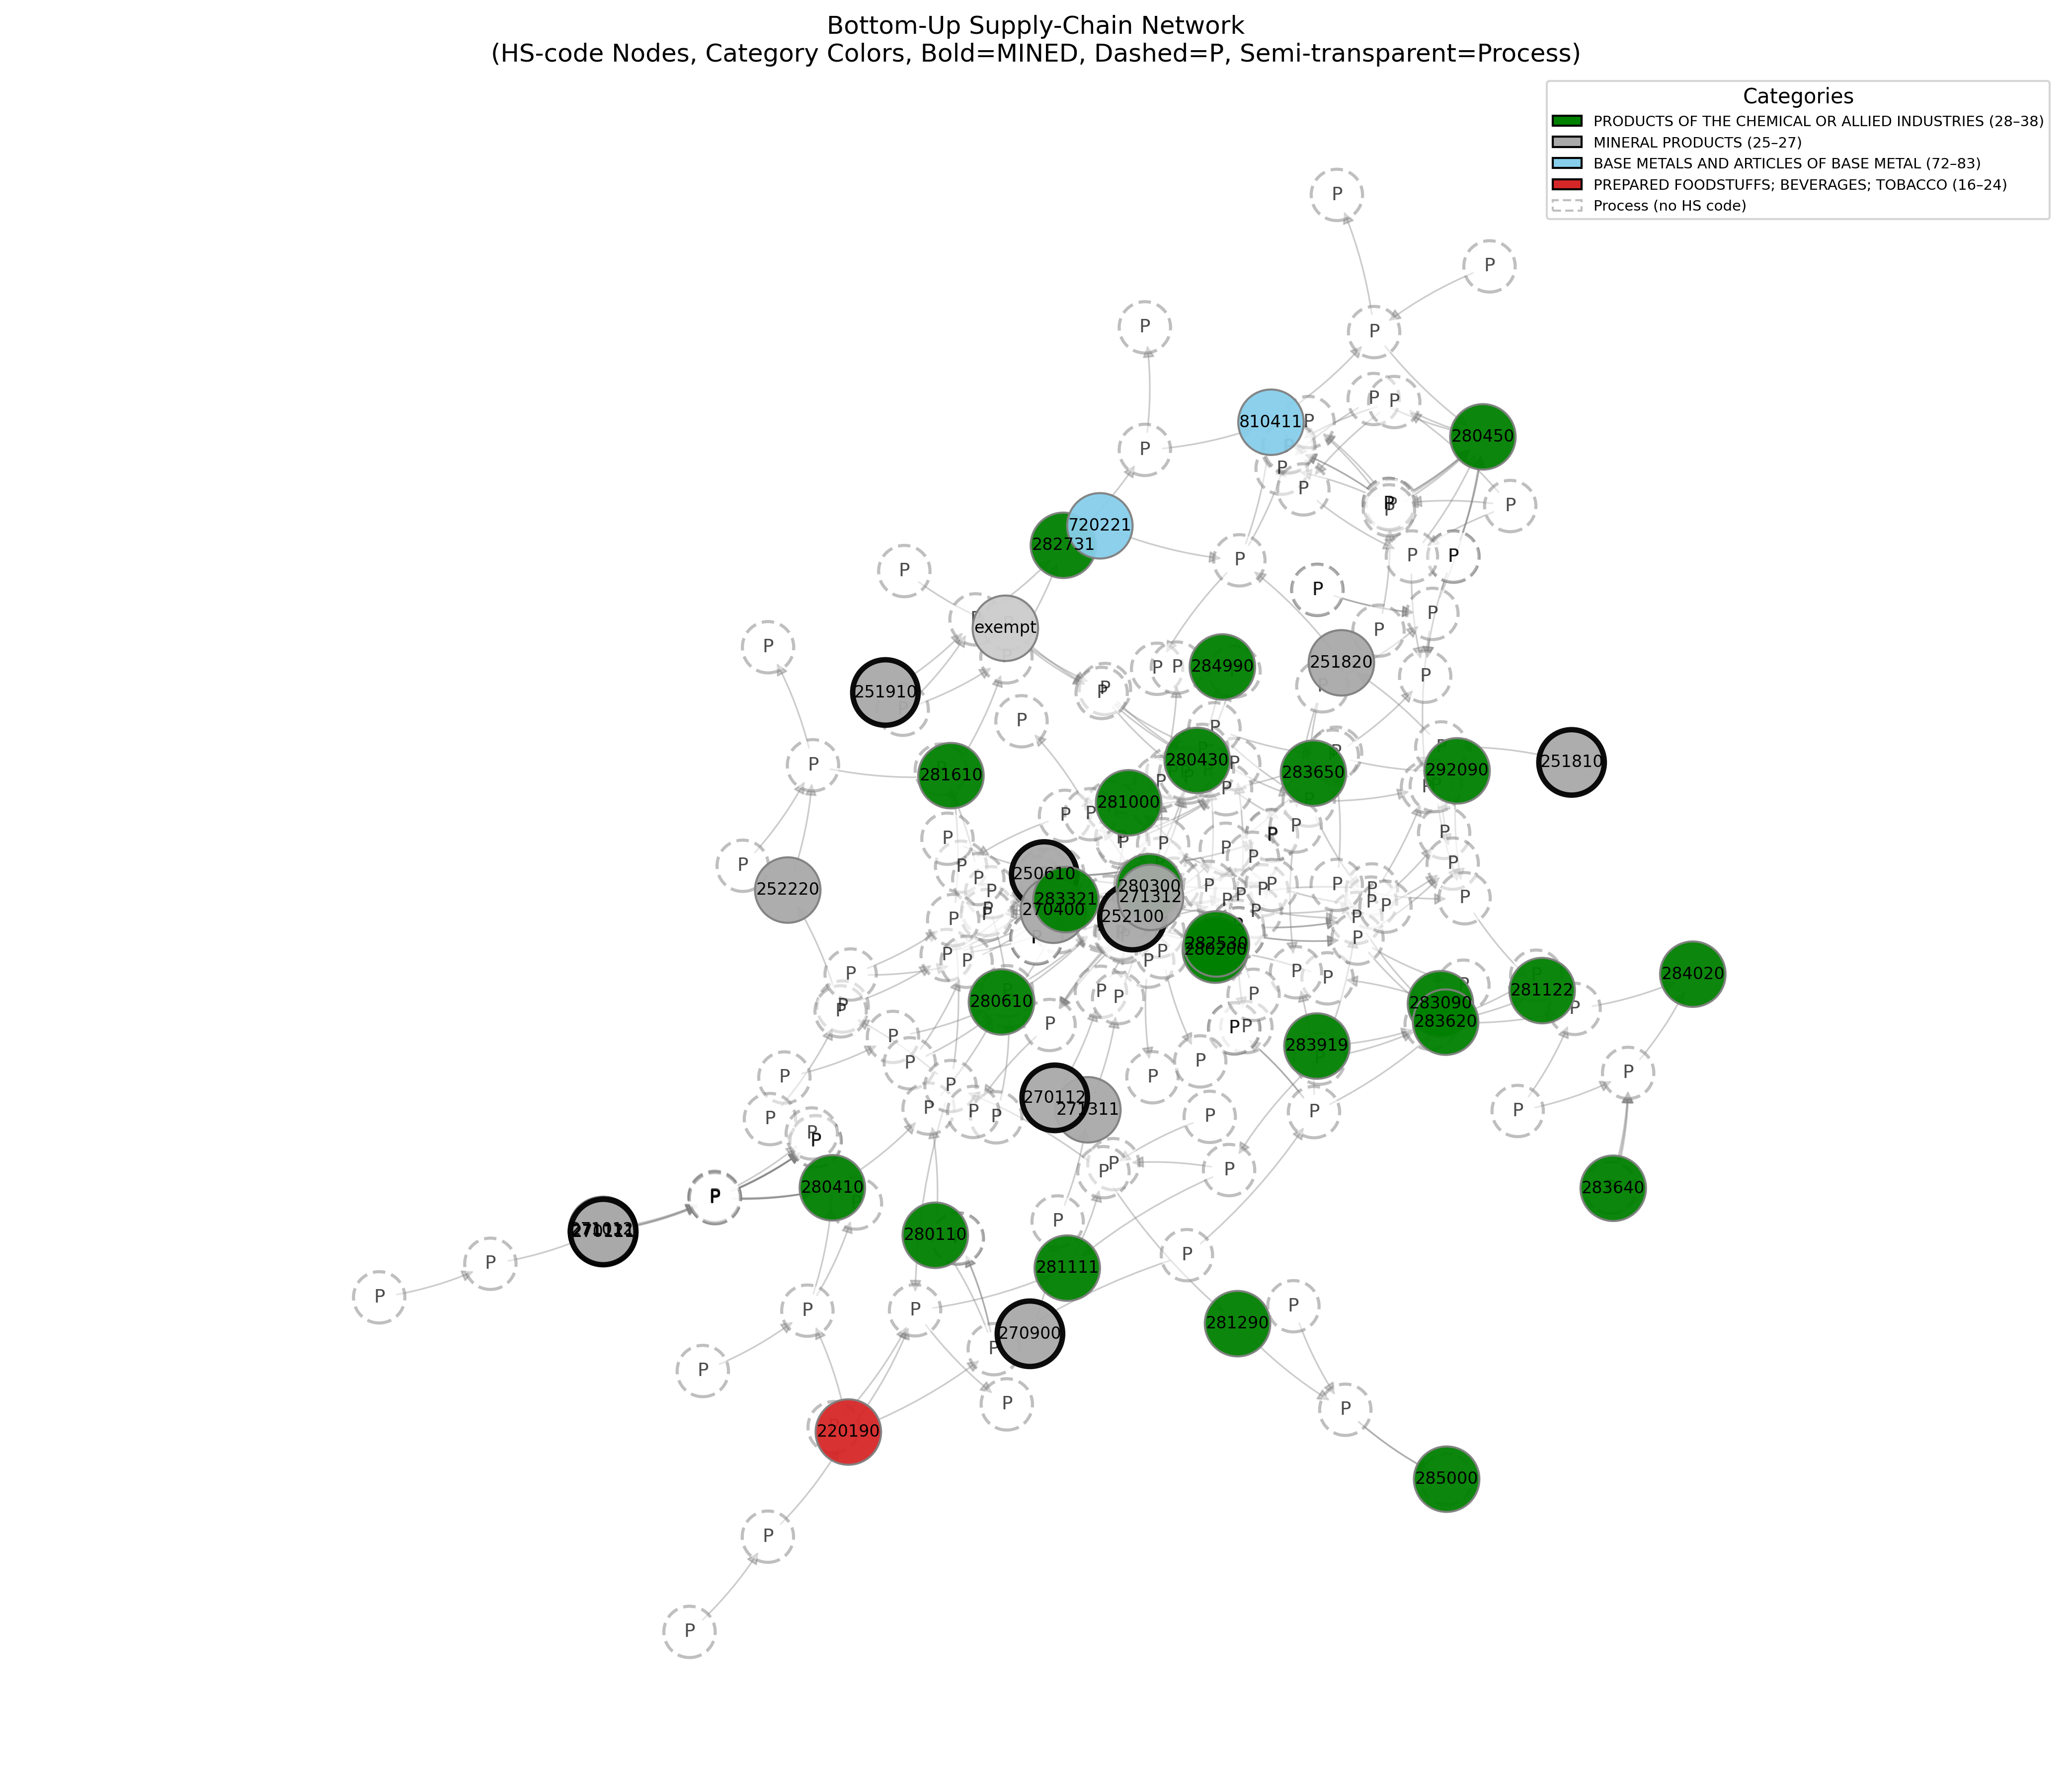
\includegraphics[width=1.0\linewidth]{images/network_analysis_network.png}
% \caption{Directed Projection of \tool{} for Boron. } 
% \label{fig:Boron-viz}
% \end{figure}


\begin{figure}[h]
    \centering
    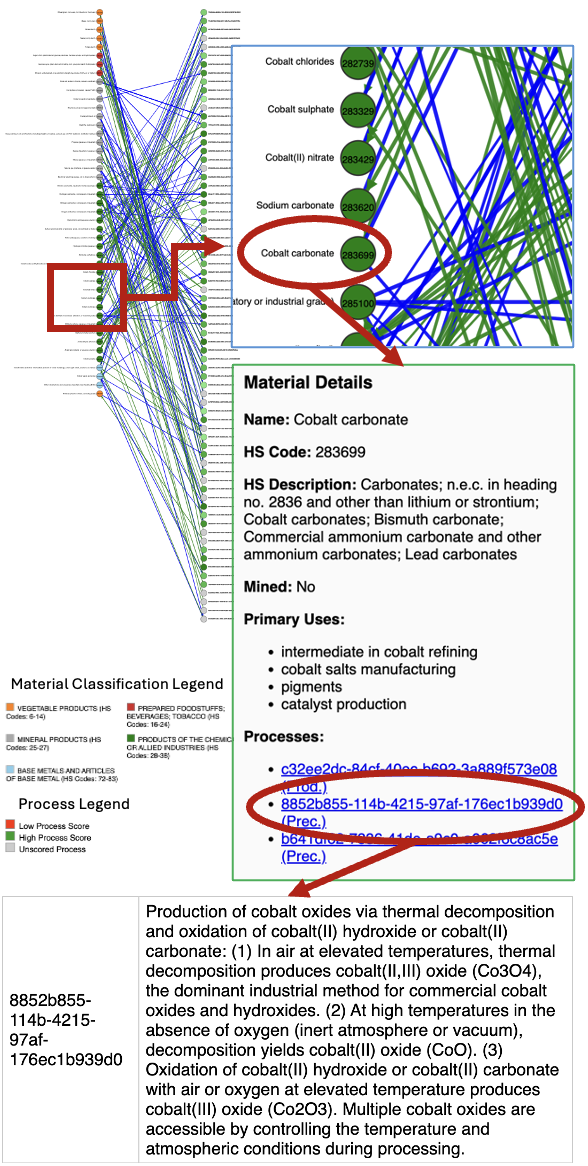
\includegraphics[width=0.9\linewidth]{images/bottom-up-vis-3.png}
    \caption{Network Graph Visualization and Interaction.  Material Nodes (left) are shown connected to one or more process hyperedges (right). Blue lines show the inputs to the processes.  Green lines show the outputs of the process.}
    \label{fig:netgraph-details}
\end{figure}

Using the generated vertices and hyperedges, a hypergraph was constructed for each material. 
Figure~\ref{fig:netgraph-details} shows a visualization of the generated hypergraph for Boron. The hypergraph $\Hcal(M,E)$ is visualized as a directed bipartite graph $G(V_1, V_2, E_G)$ with the materials as the nodes on the left and the processes (hyperedges in the original hypergraph) as the nodes on the right. For each material $m \in M$, we introduce a node $v_m \in V_1$ in $G$. For each hyperedge $e = (e_s, e_t) \in E$, we introduce a node $v_e \in V_2$ in $G$. For every material in the source
set of $e$, i.e., for each $m \in e_s$, we add a directed edge $(v_m, v_e)$ to $E_G$. Similarly, for every material in the target
set of $e$, i.e., for each $m \in e_t$, we add a directed edge $(v_e, v_m)$ to $E_G$. The visualization also zooms in on a few
nodes to show details.
% Figures \ref{fig:Boron-viz} and \ref{fig:netgraph-details} show two different visualizations of the generated hypergraphs for Boron. Figure \ref{fig:Boron-viz}, a directed projection of the multi-hypergraph,  is a simplified graph derived from the full directed hypergraph representation of the material processing network. In the original hypergraph, each process connects multiple precursor materials (inputs) to one or more product materials (outputs). The directed projection translates that structure into a standard directed graph, where edges represent directional relationships between entities—either from a material to the process that consumes it (precursor → process) or from a process to the material it produces (process → product). This projection makes it possible to apply conventional network-analysis methods (such as degree, reachability, and centrality) while still preserving the directionality and flow of transformations across materials and processes.  Figure \ref{fig:netgraph-details} presents an alternative visualization, where the material nodes are represented on the left and the processes (hyperedges) are represented as nodes on the right.  The lines between them represent precursor and product links between the two.


% $\Hcal(M, E)$, each $e=(A, B)\in E$

% $R(S) = \cup_T{\mbox{there is a sequence of hyper edges from $S$ to $T$}}$

% $(A, B), (B, C), $

% $R(v) = \cup_{S, v\in S} R(S)$

\subsubsection{Vertices (Nodes): Materials}

Each vertex/node represents a distinct material and contains the following data: a \textbf{canonical name} that provides standardized identification, a \textbf{six-digit HS code} for global trade classification, and a \textbf{mined status} flag indicating whether the material is extracted from natural sources or represents an intermediate compound. Additional attributes include \textbf{aliases} for alternative names and trade designations, \textbf{primary downstream uses} describing industrial applications, and the \textbf{HS code description} providing the official classification text. This node structure connects materials across industrial domains, trade categories, and chemical classification systems. Figure \ref{fig:netgraph-details} shows an example of what a material node looks like under Material Details. 

\subsubsection{Hyperedges: Transformation Processes}

Transformation processes are represented as hyperedges that link multiple input materials to multiple output materials. Each hyperedge contains a \textbf{descriptive narrative} of the transformation process, \textbf{scale information} indicating industrial, commercial, or laboratory operation, and \textbf{precursor and product lists} linked to material nodes via HS codes. Associated references include \textbf{URLs}, \textbf{source quality scores} reflecting domain credibility, \textbf{content relevance scores} indicating process support, and a derived \textbf{process confidence score}. Hyperedges with identical input and output HS code sets are de-duplicated while retaining all supporting references.

\subsection{Structural Analysis}
\label{sec:criticality}
% \subsubsection{Traceability and Connectivity}

\begin{figure}
    \centering
% 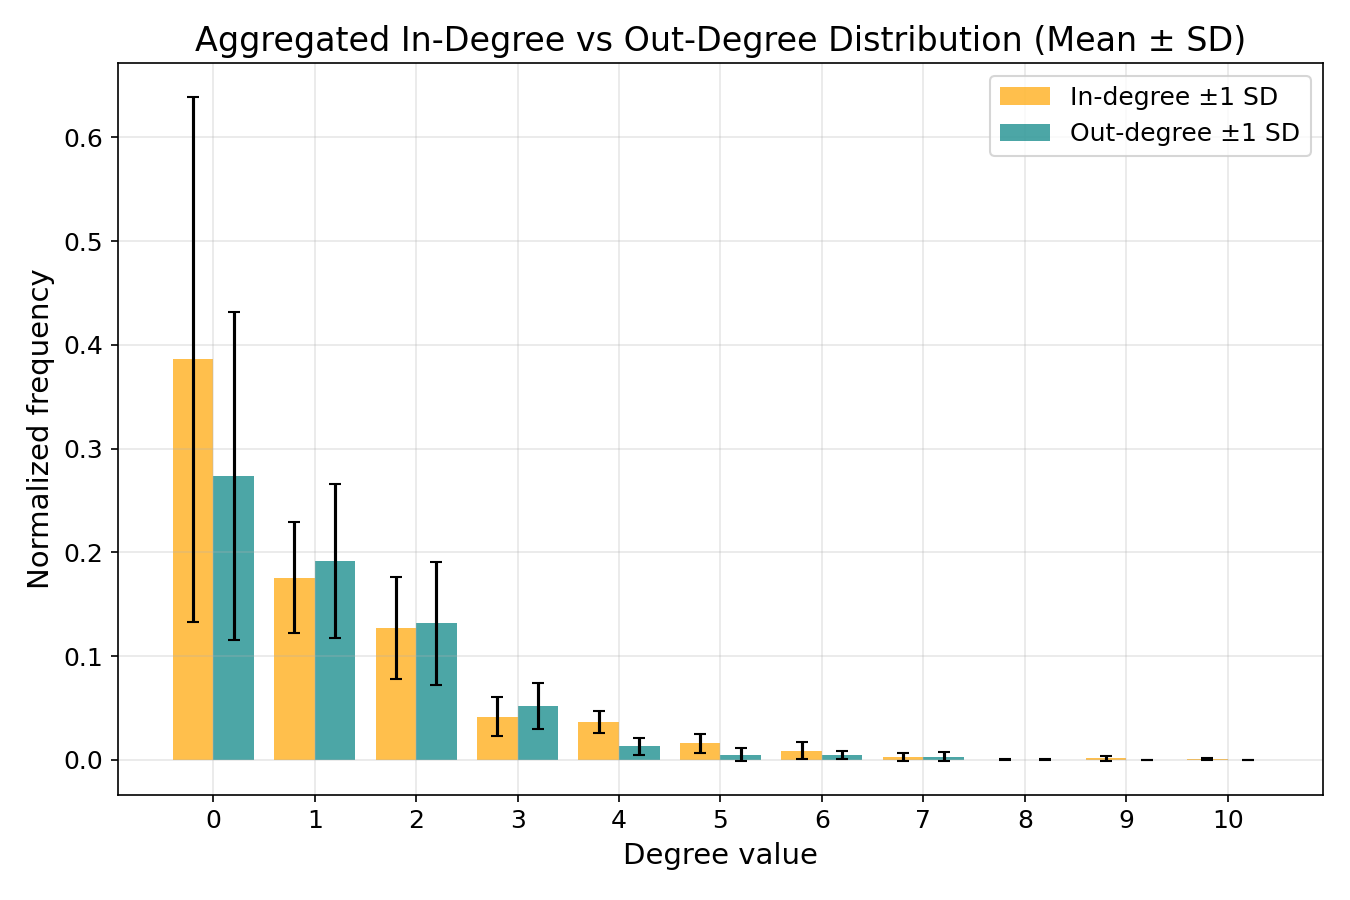
\includegraphics[width=0.9\linewidth]{images/summary_degree_comparison_avgdist.png}
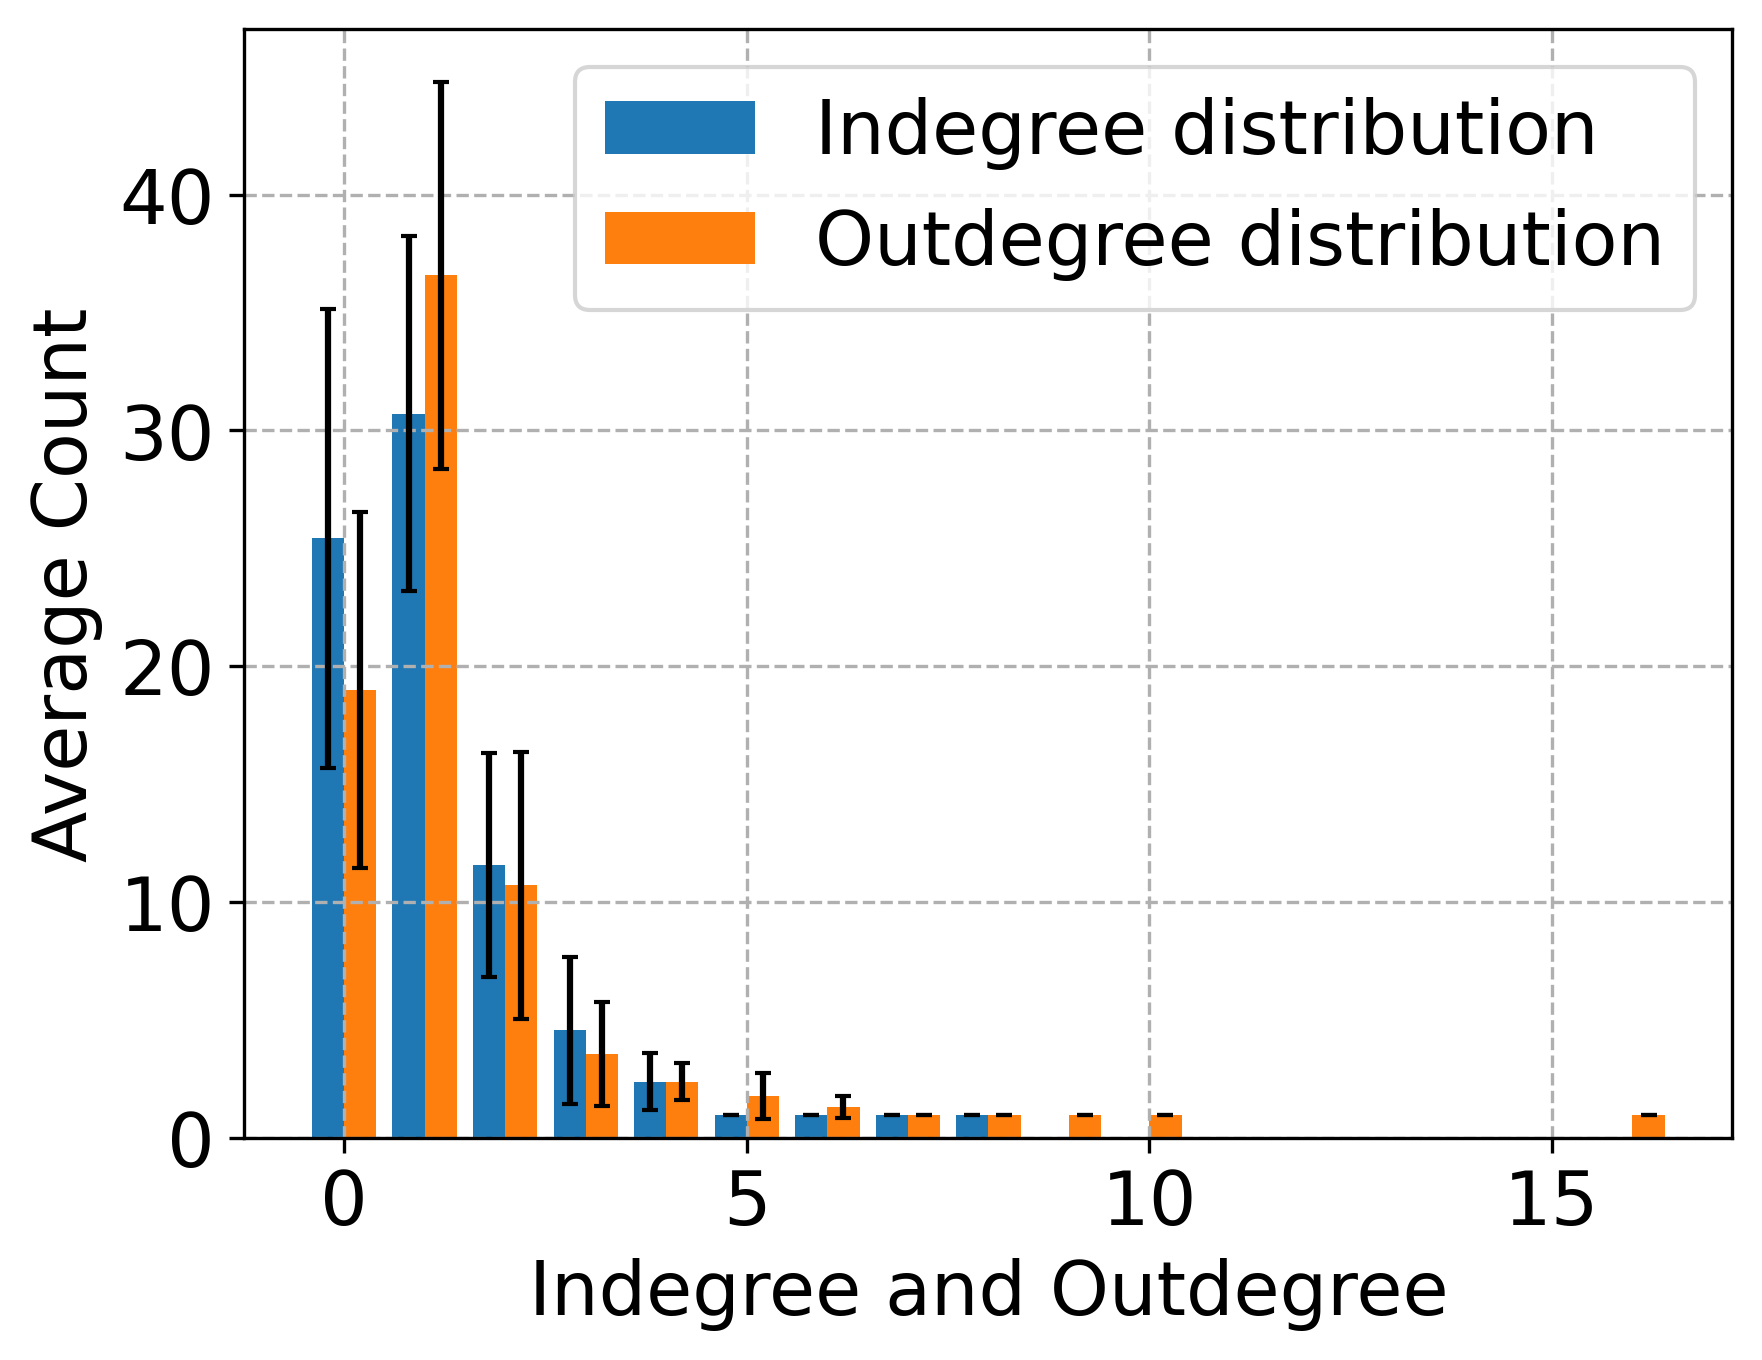
\includegraphics[width=0.9\linewidth]{images/boron_degree_distributions.png}
\caption{In- and Out-degree distributions of \tool{} for Boron, computed from 7 independently generated instances. Error bars show one standard deviation.}
\label{fig:degree}
\end{figure}


We analyze some of the fundamental network properties of the \tool{}s for Boron.
% degree, reachability and centrality distributions.
% High values with respect to these metrics can indicate high criticality for these processes. 
The most basic metric is the degree distribution.
For a node $v\in M$, we define the out-degree $d_{out}(v)=|\{e=(e_s, e_t)\in E: v\in e_s\}|$ as the number of hyperedges for which it is part of the source.
Similarly, we define the in-degree $d_{in}(v)=|\{e=(e_s, e_t)\in E: v\in e_t\}|$.
Figure~\ref{fig:degree} shows the in- and out-degrees of nodes in \tool{}s for Boron. 
Only a small fraction of nodes are involved in multiple processes, and are critical from that perspective.

The hypergraph structure supports bidirectional traversal: downstream materials can be traced to their mined origins, and extracted materials can be followed to derived intermediates and products. 
The network reveals parallel pathways to identical products, indicating potential substitution routes and alternative production methods. 
Bottleneck processes appear as hyperedges connecting otherwise separate network components. This structure supports both pathway analysis and quantitative assessment of connectivity, redundancy, and material criticality.


% \subsection{Analysis of material criticality}

We now define a notion of criticality for materials that constitute a \tool{}. The intuitive idea is as follows. Each \tool{} is
constructed for a given base material, e.g., Boron, which we denote as $m_{base}$. The \tool{} describes the set of processes (hyperedges) by which $m_{base}$,
in combination with other raw materials, can be used to generate new materials. The total set of materials that can be generated
in this way is the \textit{reach} of $m_{base}$ in the \tool{} hypergraph. The notion of reach is similarly defined for any
material $m \in M$.

The criticality of any other material in the \tool{} is the reduction in the number of materials that can be generated if we
remove this material from the \tool{}. Thus, it is the reduction in the reach of $m_{base}$ when the other material
is removed. From a policy perspective, removing a material could correspond to banning the production and use of that material. 
The impact of the policy is the criticality of the removed material, as it quantifies the cascading effect of removing that 
material on the production of other materials. We formalize these notions below.

\begin{definition}
\label{def:reach}
\textbf{Precursor Set.}
Given a \tool{} $\Hcal(M, E)$, where each hyperedge $e \in E$ has a source set $e_s$ and a target set $e_t$, we define the precursor set $\mathtt{Pre} = \bigcup_e e_s - \bigcup_e e_t$ to be the set of materials which appear only in hyperedge sources.
\end{definition}

\begin{definition}
\label{def:reach}
\textbf{Reachable set.}
Given a \tool{} $\Hcal(M, E)$ and a set $m_{start} \subseteq M$, a material $m_i$ is considered reachable if it is in the
target set of a hyperedge whose source set contains only materials that are in $m_{start}$ or are themselves reachable. The 
reachable set, $R(m_{start}, \Hcal)$ is the set of all nodes that are reachable from $m_{start}$ in $\Hcal$.
\end{definition}

\begin{definition}
\label{def:criticality}
\textbf{Criticality.}
Given a \tool{} $\Hcal(M, E)$ and a set $m_{start} \subseteq M$, the criticality of a material $m_i$ is defined as, 
\begin{align}
\nonumber
c(m_i, m_{start}, \Hcal) = |R(m_{start}, \Hcal)| - |R(m_{start}\setminus m_i, \Hcal \setminus m_i)|,
\end{align}
i.e., it is the reduction in the 
size of the reachable set when $m_i$ is removed.
\end{definition}

In our analysis of criticality, we always set $m_{start} = m_{base} \cup \mathtt{Pre}$. For each \tool{}, we compute $c(m_i, 
m_{start}, \Hcal) \forall m_i \in M$ (except for $m_{base}$ itself). Table~\ref{table:criticality} shows
the top 3 most critical materials for multiple \tool{}s. For a \tool{}, its \textbf{criticality list} is the set $M$ of 
its materials, ordered from most critical to least critical. Note that this list is partially ordered, as several materials can
have the same criticality.

\begin{table}[h]
%\vspace{-0.3in}
%\centering
\caption{Top 3 critical materials in each \tool{}. In each case, $m_{base}$ is written in bold. The criticality value
for $m_{base}$ is $R(m_{base} \cup \mathtt{Pre}, \Hcal)$.}
\begin{center}
% \begin{tabular}{|r|c|} \hline
\begin{tabular}{|R{0.8\linewidth}|l|} \hline
\toprule
Material [HS Code] & Criticality \\ 
\midrule
\textbf{Elemental Boron [284520]} & \textbf{73} \\
Hydrogen (byproduct) [280410] & 12 \\
Oxygen [280440] & 9 \\
Fumed silica [281122] & 8 \\
% Soda Ash (Sodium Carbonate) [283620] & 8 \\
% Silicon tetrachloride [281230] & 7 \\
\midrule
\textbf{Cobalt ore and concentrates [260500]} & \textbf{61} \\
Sodium Chloride (in brine solution) [250100] & 8 \\
Sodium Hydroxide (caustic soda) [281512] & 6 \\
Water (distilled or deionized) [285100] & 5 \\
% Sulfuric acid [280700] & 5 \\
% Hydrogen (elemental, compressed or liquefied) [280410] & 5 \\
\midrule
\textbf{Gallium in ores and concentrates [260600]} & \textbf{53} \\
Lithium bromide [282759] & 7 \\
Lithium chloride [282720] & 6 \\
Carbon monoxide [281121] & 5 \\
% Natural gas [271121] & 5 \\
% Methyllithium [284530] & 4 \\
% \midrule
% \textbf{Quartz (natural silica, silicon ore) [250610]} & \textbf{18} \\
% Silicon (not less than 99\% purity) [280469] & 6 \\
% Sodium silicates [283911] & 5 \\
% Silica sand [250510] & 5 \\
% Silicon dioxide (synthetic silica gel) [281122] & 4 \\
% Ferro-silico-chromium [720250] & 3 \\
\midrule
\textbf{Germanium metal, unwrought [811292]} & \textbf{40} \\
Coke (coal-derived, industrial grade) [270400] & 6 \\
Calcium carbide, industrial grade [284910] & 6 \\
Sawdust or wood shavings [440149] & 5 \\
% Carbon monoxide [282410] & 4 \\
% Lime (Calcium oxide, quicklime) [252210] & 4 \\
\bottomrule
%\hline\end{tabular}
\end{tabular}
\end{center}
\label{table:criticality}
\end{table}

\subsection{Sensitivity Analysis} 
% \samarth{Changed from ``Disruption'' to ``Sensitivity''}

To study the sensitivity of the criticality analysis to the stochasticity in the \tool{} generation process, we
formalize a method for sensitivity analysis. Our approach is quite general, and the criticality analysis can be replaced with 
other kinds of analysis easily.

We assume that a \tool{} $\Hcal(M, E)$ is a sample from an underlying distribution over \tool{}s, $\Phi$. Suppose that we
are interested in computing a function, $F(\Hcal)$, from $\Hcal$, which may be a relevant measure for some policy analysis.
Examples of $F$, based on Section~\ref{sec:criticality}, might be the most critical material, the ordering of the criticality 
list, the distribution of orders in the criticality list (i.e., how many materials are at each level of criticality), etc. We
would like to understand the sensitivity of $F$ to the stochastic variability in the network generation process. We quantify
this as a measure of dispersion of $F$ from its expected value according to $\Phi$. When $F$ is continuous valued, its 
expectation is $E(F) = \sum_\Hcal F(\Hcal)\Phi(\Hcal)$, and sensitivity would be, e.g., its standard deviation $\sigma(F)$ with 
respect to $E(F)$. In practice, since $\Phi$ is unknown, we would use the sample mean, $\overline{F}$, and the sample standard
deviation, $s(F)$.

To generalize this to criticality lists, we use a ranked list aggregation method instead of $\overline{F}$ and a 
measure of agreement over ranked lists instead of $s(F)$. Specifically, we use Borda Count (BC) to generate an
aggregate criticality list, where the score assigned to a list item is its criticality. In the BC method, scores for 
each item are aggregated by summing across lists, and the resulting list is sorted in descending order. For measuring 
the agreement between the aggregate list and each of the individual criticality lists, we use the Rank-biased Overlap 
(RBO)~\cite{webber10rbo} concordance measure.

RBO is an appropriate measure for our application for two reasons: it does not require the lists to have the same lengths or
identical sets of elements, and it allows biasing the measure towards comparing the top-ranked elements through its 
\textit{persistence} parameter (higher values correspond to higher emphasis on the top-ranked elements). Our criticality lists
can have different sets of elements for different samples of the network generated for the same base material. Criticality also
tends to be low for many nodes in the \tool{} and high for relatively few nodes. This is borne out by the distribution of 
criticality scores from the aggregate criticality list shown in Figure~\ref{fig:criticality}. Thus, emphasizing the top-ranked 
elements makes sense. RBO measures the overlap between two lists iteratively at successive depths. Its value ranges from 0 to 
1, where 0 indicates that the lists are disjoint and 1 indicates that they are identical.

We generated seven instances of the Boron \tool{} and computed the criticality list for each of them with $m_{base} = 284520$ 
(elemental boron) in each case. We then used the BC method to construct the aggregate list and computed RBO for each criticality
list with the aggregate list. Persistence was set to 0.98, which corresponds to $\sim50\%$ of the weight being assigned to the top 
35 elements in the lists. The mean value of RBO was 0.462 and its standard deviation was 0.03. This shows that, while the 
criticality lists are not identical, they have good agreement to a significant depth. The low standard deviation shows that all
the criticality lists have about the same overlap with the aggregate list.

\begin{figure}
    \centering
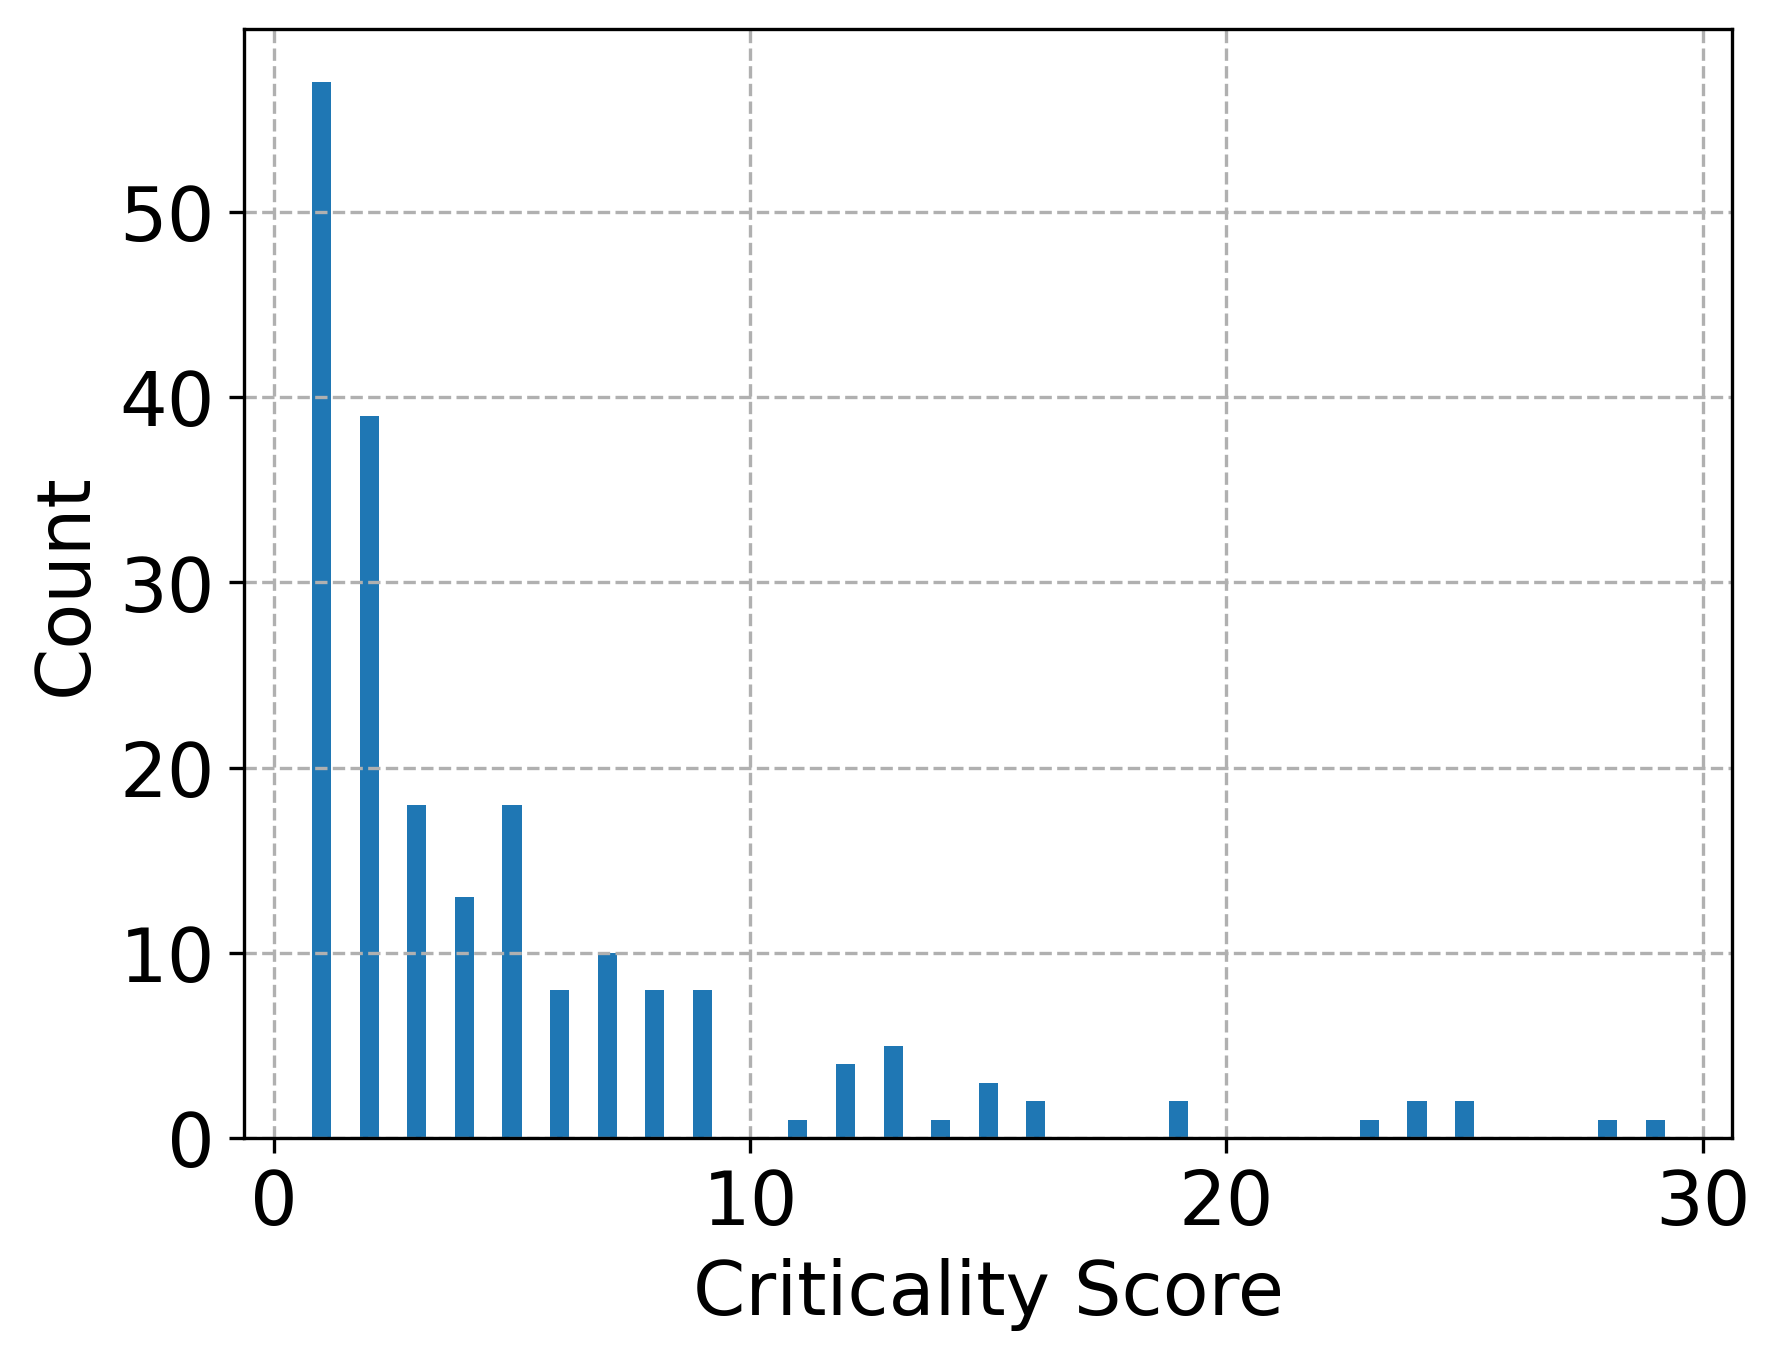
\includegraphics[width=0.9\linewidth]{images/boron_criticality_distribution.png}
\caption{The distribution of criticality scores from the aggregate criticality list for Boron. Note that BC aggregates by summing, so the values here are the sums of the criticalities from the seven criticality lists.}
\label{fig:criticality}
\end{figure}


% In order to study the effects of disruptions on \tool{}s, we present a formalization of disruption analysis.
% This formalization looks specifically at disruptions to \textit{processes} and potential downstream and second-order effects.
% In this model, we additionally endow each material with an availability state $s(m_i) \in [0,1]$, where a fully available material has state $1$, and a fully unavailable material has state $0$.
% We additionally denote by $\varphi(m_i) \subset E$ the set of processes for which $m_i$ is an output, and by $p_{in}$ the set of inputs for process $p$.

% We define a disruption as a flow-based process through the MEG. 
% We update the state of each material according to the following rule.
% For each material $m$, we say that the state of $m$, $s(m) = \max_{p \in \varphi(m)}\min_{m' \in p_{in}}s(m')$. 
% That is to say, each material is disrupted by the process with the least restrictive amount of disruption.
% In this disruption model, we assume that each process is equally capable; that is, if processes $p_1$ and $p_2$ both produce output $m$, they produce equal amounts of $m$. 
% In the initial state, we model a process disruption for process $p$ as setting the state of each $m \in p_{out}$ to be $\frac{|\varphi(m)| - 1}{|\varphi(m)|}$; that is, each output of the process is decreased by the amount created by that output. 

% Because MEGs may have cycles, this update model must propagate through the MEG, until an equilibrium is reached. 
% We say that the equilibrium state is the final disruption analysis, and specifically look at the effect on the material state. 
% \gsh{Open questions: 1. When is an equilibrium guaranteed to exist? 2. Can we efficiently compute the equilibrium state?}


\subsection{Disruption Analysis}
Using the Boron \tool{} and Comtrade data~\cite{UNComtrade2024} for 2024, we
assess how disruptions in countries dominating the export of key raw
or intermediary materials (HS 6-digit level) cascade through
downstream technologies. 
The United Nations Comtrade Database is the official global repository of detailed international trade statistics collected and published by the United Nations. It provides import and export data reported by more than 200 countries and territories, organized by commodity categories and trading partners. The database enables researchers, policymakers, and businesses to analyze global trade flows, economic dependencies, and supply chain dynamics across time and regions.

For each HS 6-digit code in the MEKH, we identify the top supplier using UN Comtrade trade values and apply a 60\% dominance threshold, i.e. the leading exporter must account for at least 60\% of
global exports of that HS code. We then simulate a disruption scenario
in which the dominant supplier halts all exports of that material, and
evaluate the downstream effects on dependent HS codes within the Boron \tool{}. Specifically, any HS codes that rely exclusively on the disrupted
precursor are considered fully removed from the network.

The analysis 
reveals that while disruptions by Mexico (HS 252922),
Norway (271121), Turkey (284011), the United States (284020), and
China (810411) do not propagate further downstream, disruptions by
Poland (HS 280200) and Turkey (HS 284019) cause significant cascading
losses. Specifically, the loss of HS 280200 eliminates five dependent
HS codes, while the disruption of HS 284019 removes
four HS codes. Additionally, the US, which controls 100\% of HS
284520, could disrupt both 284520 and its dependent HS 285000, which
lacks substitute inputs.

Overall, the results indicate that although most disruptions are
localized, a few highly concentrated supply nodes, such as Poland’s HS
280200 and Turkey’s HS 284019, pose significant downstream risks within
the boron \tool{}.
